\documentclass{article}
\usepackage{graphicx} 
\usepackage{array}
\usepackage{pgfplotstable}
\author{Omkar Oak}
\title{\vspace{-5cm} Assignment 3,4,5}
\date{23 November 2022}
\begin{document}
	\maketitle
	\section{Adding Image}
	\begin{center}
	\begin{figure}[h]
	\caption{\begin{large}Japan\end{large}}
	\vspace{5 mm}
	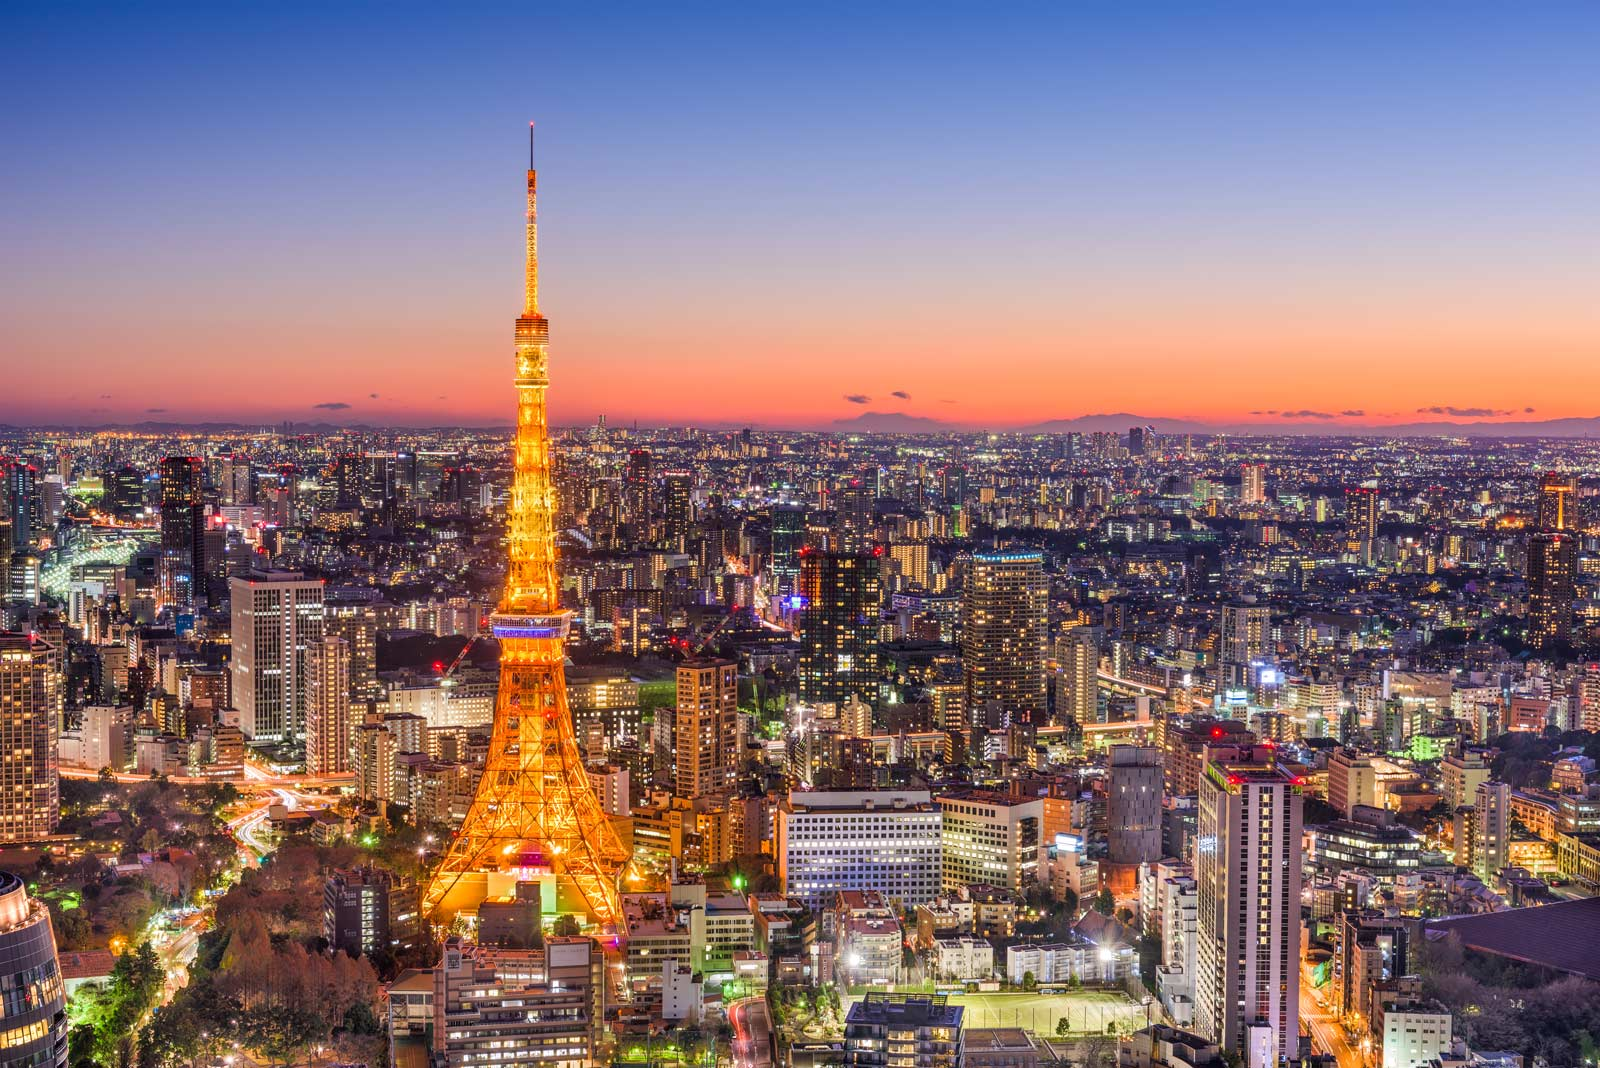
\includegraphics[width=13cm]{image1}
	\end{figure}
	\end{center}
	\section{Adding Table}
	\begin{table}[h]
	\begin{center}
	\caption{Cities of Japan}
	\vspace{5 mm}
	\begin{tabular}{|l|c|c|c|c|r|}
	\hline
	\textbf{Sr.No} & \textbf{City} & \textbf{District} & \textbf{Population}\\
	\hline
	1 & Tokyo & Tokyo City & 3,906,753,002 \\
	\hline
	2 & Osaka & Yamada ken & 3,206,453,779 \\
	\hline
	3 & Kyoto & Funigawa & 2,106,330,110\\
	\hline
	4 & Sapporo & Hokkaido & 1,020,030,000 \\
	\hline
	\end{tabular}
	\end{center}
	\end{table}
	\newpage
	
\section{Table Examples}
Study the following table and answer the questions based on it 
\cite{float}

\begin{table}[h] 
\begin{tabular}{|l|c|c|c|c|r|}
\hline
Year & \multicolumn{4}{c}{Item of Expenditure} \\ \hline
& Salary & Fuel and Transport & Bonus & Interest of Loans & Taxes\\
 \hline
 1998 & 288 & 98 & 3.00 & 23.4 & 83 \\ 
  \hline
 1999 & 342 & 112 & 2.52 & 32.5 & 108 \\ 
  \hline
 2000 & 324 & 101 & 3.84 & 41.6 & 74 \\ 
 \hline
 2001 & 336 & 133 & 3.68 & 36.4 & 88 \\ 
 \hline
 2002 & 420 & 142 & 3.96 & 49.4 & 98 \\ 
 \hline
\end{tabular}
\caption{\label{Question I} Expenditures of a Company (in Lakh Rupees) per Annum Over the given Years.}
\end{table}


\begin{enumerate}
\item The total amount of bonus paid by the company during the given period is approximately what percent of the total amount of salary paid during this period?
\item Total expenditure on all these items in 1998 was approximately what percent of the total expenditure in 2002?
\item The total expenditure of the company over these items during the year 2000 is?
\item The ratio between the total expenditure on Taxes for all the years and the total expenditure on Fuel and Transport for all the years respectively is approximately?
\end{enumerate}


\begin{table}[h]
\begin{tabular}{|l|c|c|c|c|c|r|}
\hline
	& \multicolumn{6}{c}{Subject (Max. Marks)} \\ \hline
 Student & Maths	 & Chemistry	 & Physics & Geography & History & Comp Sci \\ \hline
Ayush	& 90 & 50 & 90 & 60 & 70 & 80 \\
Aman	    & 99 & 80 & 80 & 40 & 80 & 70 \\
Sajal	& 90 & 60 & 70 & 70 & 90 & 70 \\
Rohit	& 80 & 65 & 80 & 80 & 60 & 60 \\
Muskan	& 80 & 65 & 85 & 95 & 50 & 90 \\
Tanvi	& 70	 & 75 & 65 & 85 & 40 & 60 \\
Tarun	& 65 & 35 & 50 & 77 & 80	& 80 \\
\hline
\end{tabular}
\end{table}
\noindent \cite{theory} 
The above table gives the percentage of marks obtained by seven students in six different subjects in an examination. \\ 
\textit{The numbers in the brackets give the maximum marks in each subject.}

\begin{enumerate}
\item What are the average marks obtained by all the seven students in Physics? (rounded off to two digit after decimal)
\item The number of students who obtained 60\% and above marks in all subjects is?
\item What was the aggregate of marks obtained by Sajal in all the six subjects?
\item In which subject is the overall percentage the best?
\item What is the overall percentage of Tarun?
\end{enumerate}

\section{Table from CSV}
\subsection*{Question I}
\begin{table}[h]
  \begin{center}
    \caption{Autogenerated table from .csv file.}
    \label{table1}
    \pgfplotstabletypeset[
	col sep=comma,
	columns = {Roll Number, Science, Computer, Maths, History}
]{data1.csv} % filename/path to file
  \end{center}
\end{table}
\begin{enumerate}
\item What is the total marks obtained by the student in history and computer together?
\item Who scored the lowest marks in all the subjects?
\item What is the median mark of the students in mathematics?
\item What is the range of marks obtained by the students in history?
\end{enumerate}
\pagebreak


\begin{thebibliography} {}
\bibitem{book} “Digital Design” M Morris Mano, 5th Edition, 2013, Pearson Education, ISBN-10: 0-13-277420-8 / ISBN-13: 978-0-13-277420-8
\bibitem {float} “Discrete Mathematics”, Lipschutz, Lipson, 2nd Edition, 1999, Tata McGraw-Hill, ISBN: 007 463710X
\bibitem{real} Real Number Symbol in LaTeX, $https://www.physicsread.com/latex-real-number/$
\bibitem {theory}“Theory of computer science”, E. V. Krishnamurthy, 2004, Affiliated East Press Publications, ISBN-10: 038791255X / ISBN-13: 978-0387912554.

\end{thebibliography}
\end{document}